\documentclass[runningheads]{llncs}

\usepackage{amsmath,amssymb,amsfonts}
\usepackage{algorithmic}
\usepackage{algorithm}
\usepackage{graphicx}
\usepackage{textcomp}
\usepackage{xcolor}
\usepackage{booktabs}
\usepackage{microtype}
\usepackage{url}
\usepackage{tikz}
\usepackage{multirow}
\usepackage{enumitem}
\usepackage{etoolbox}

% --- Page compression: tighter floats, captions, sections ---
\setlength{\textfloatsep}{5pt plus 1pt minus 1pt}
\setlength{\floatsep}{3pt plus 1pt minus 1pt}
\setlength{\intextsep}{3pt plus 1pt minus 1pt}
\setlength{\abovecaptionskip}{2pt}
\setlength{\belowcaptionskip}{1pt}
\setlength{\abovedisplayskip}{4pt plus 1pt minus 1pt}
\setlength{\belowdisplayskip}{4pt plus 1pt minus 1pt}
\setlist{nosep, topsep=1pt, partopsep=0pt, itemsep=0pt}
\renewcommand{\topfraction}{0.95}
\renewcommand{\bottomfraction}{0.95}
\renewcommand{\textfraction}{0.05}
\renewcommand{\floatpagefraction}{0.85}

% --- Compact bibliography ---
\let\oldthebibliography\thebibliography
\let\endoldthebibliography\endthebibliography
\renewenvironment{thebibliography}[1]{%
  \begin{oldthebibliography}{#1}%
    \scriptsize
    \setlength{\itemsep}{0pt}%
    \setlength{\parsep}{0pt}%
    \setlength{\parskip}{0pt}%
}{%
  \end{oldthebibliography}%
}
\usetikzlibrary{shapes.geometric, arrows.meta, positioning, fit, backgrounds, calc}

\begin{document}

\title{Defending Autonomous LLM Agents Against Indirect Prompt Injection: Semantic Boundary Enforcement and Multi-Signal Voting for Data-Channel Attack Detection}

% Double-Blind Compliance
\author{Anonymous Author(s)}
\institute{Affiliation Withheld for Double-Blind Peer Review}

\maketitle

\begin{abstract}
Autonomous Large Language Model (LLM) agents combine foundational reasoning with external tool execution, exposing critical workflows to untrusted external data such as incoming emails, scraped web content, and third-party API payloads. This interface introduces indirect prompt injection (IPI) vulnerabilities, where adversaries manipulate external data to hijack the agent's execution flow. Existing defensive approaches largely rely on stateless ingress prompt classifiers, overlooking the fundamental confusion between instructions and data channels, while neglecting egress output sanitization and multi-signal corroboration. 
In this paper, we propose a multi-layered defense architecture specifically designed to counteract data-channel IPI attacks against autonomous agents. The central scientific contribution is a semantic-boundary enforcement and family-based multi-signal aggregation framework for detecting and containing indirect prompt injections across data channels. Our architecture introduces: (1)~\textit{InstructionBoundaryDetector}, a structural parser and imperative pattern analyzer that enforces semantic boundaries between benign data containers and embedded instructions; (2)~\textit{EmailVectorDetector}, a specialized heuristics engine targeting multi-vector indirect injections across communication channels; (3)~\textit{VotingAggregator}, a multi-signal decision engine employing family-based signal grouping to isolate structural boundary violations from behavioral anomalies while enforcing a strict anti-feedback loop invariant and decision tier monotonicity; and (4)~\textit{ContextSanitizer} coupled with \textit{DataRedactor}, an egress defense pipeline executing ML-guided context remediation and 8-pattern secret/PII redaction before data enters the agent's context. 
Evaluated on an AgentDojo-derived evaluation corpus comprising 29,038 operational records across 21,825 agent sessions, our system achieves an Attack Block Success Rate (ABSR) of 84.31\% and a Session-level ABSR of 89.44\%---a $3.39\times$ higher Session-level ABSR than our re-implementation of SafeHarness under the same evaluation protocol---with a steady-state false positive rate of 8.41\%. In targeted red-teaming across 20 adversarial evasion scenarios, the system intercepts 19 out of 20 attacks (95.0\%), demonstrating robust defense-in-depth across data-channel threats.

\keywords{LLM Agent Security \and Indirect Prompt Injection \and Instruction Boundary Enforcement \and Data-Channel Attack \and Multi-Signal Intrusion Detection \and Egress Sanitization}
\end{abstract}

% =========================================================================
% SECTION 1: INTRODUCTION
% =========================================================================
\section{Introduction}
\label{sec:intro}

The integration of Large Language Models (LLMs) into autonomous agent frameworks---exemplified by ReAct~\cite{yao2023react}, AutoGen~\cite{wu2024autogen}, and enterprise task automations---has marked a paradigm shift in systems engineering. The foundational model functions as a centralized cognitive controller with tool execution, file system, web retrieval, and communication privileges, dramatically increasing the attack surface from passive content safety to active runtime protection~\cite{owasp2023,nist2023}.

Foremost among emerging vulnerabilities is \textit{Indirect Prompt Injection} (IPI)~\cite{greshake2023not,agentdojo2024}. Unlike direct jailbreaking, indirect injection occurs over secondary data channels: an attacker embeds malicious directives into documents, emails, web pages, or database records that the agent retrieves during normal operation. When ingested into the context window, the model's unified token stream fails to distinguish system directives from passive data, enabling unauthorized API calls, data exfiltration, and system compromise.

\begin{figure}[t]
\centering
\resizebox{\columnwidth}{!}{%
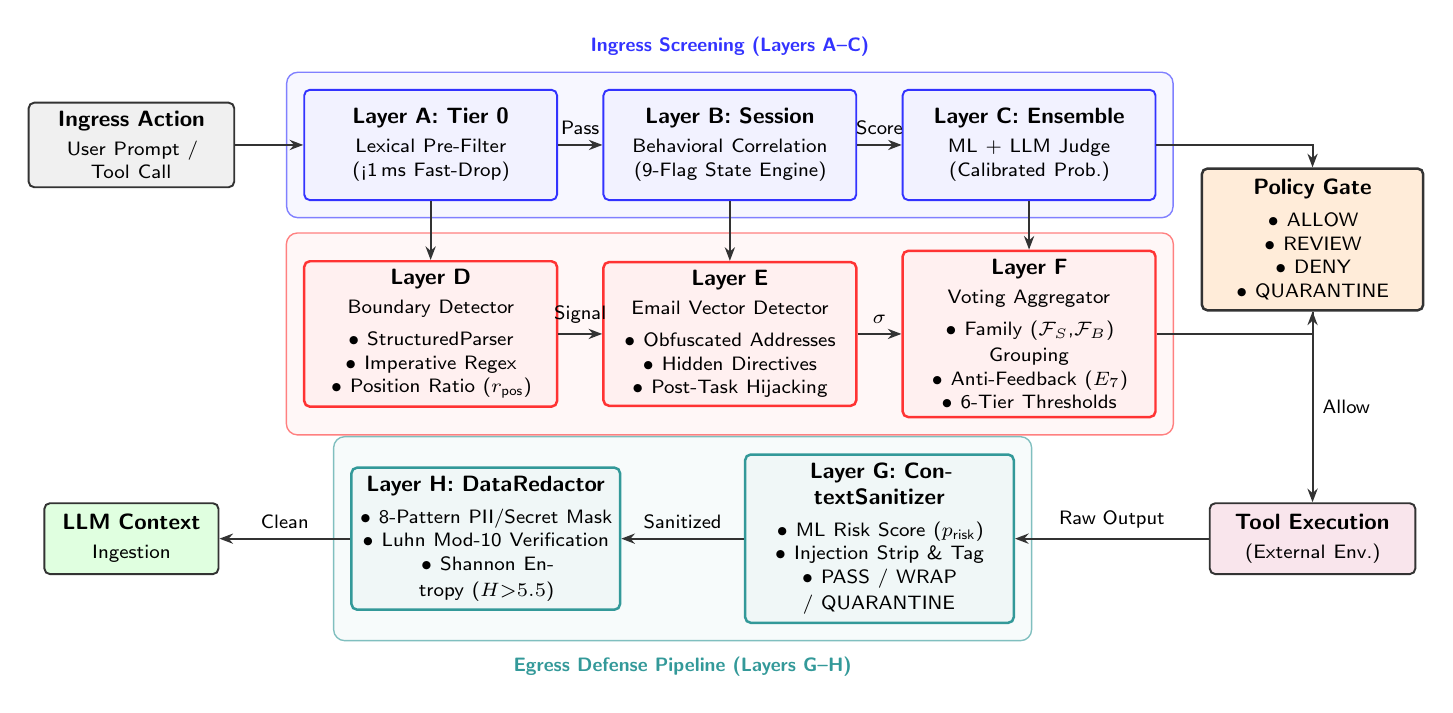
\begin{tikzpicture}[
    every node/.style={font=\sffamily\footnotesize},
    box/.style={rectangle, draw=black!80, rounded corners=2pt, line width=0.7pt,
                align=center, fill=white, inner sep=3pt, text width=2.8cm, minimum height=0.9cm},
    layerbox/.style={rectangle, draw=blue!80, fill=blue!5, line width=0.7pt,
                     rounded corners=2pt, inner sep=3pt, align=center, text width=3.0cm, minimum height=1.4cm},
    novelbox/.style={rectangle, draw=red!80, fill=red!6, line width=0.9pt,
                     rounded corners=2pt, inner sep=3pt, align=center, text width=3.0cm, minimum height=1.4cm},
    egressbox/.style={rectangle, draw=teal!80, fill=teal!6, line width=0.9pt,
                      rounded corners=2pt, inner sep=3pt, align=center, text width=3.2cm, minimum height=1.4cm},
    arrow/.style={-{Stealth[scale=0.8]}, line width=0.7pt, draw=black!80},
    lbl/.style={font=\sffamily\scriptsize}
]

% === Row 1: Ingress Screening ===
\node[box, fill=gray!12, text width=2.4cm] (input) at (0, 4.2)
    {\textbf{Ingress Action}\\[1pt]{\scriptsize User Prompt /}\\[-1pt]{\scriptsize Tool Call}};

\node[layerbox] (la) at (3.8, 4.2)
    {\textbf{Layer A: Tier 0}\\[1pt]{\scriptsize Lexical Pre-Filter}\\[-1pt]{\scriptsize (<1\,ms Fast-Drop)}};

\node[layerbox] (lb) at (7.6, 4.2)
    {\textbf{Layer B: Session}\\[1pt]{\scriptsize Behavioral Correlation}\\[-1pt]{\scriptsize (9-Flag State Engine)}};

\node[layerbox] (lc) at (11.4, 4.2)
    {\textbf{Layer C: Ensemble}\\[1pt]{\scriptsize ML + LLM Judge}\\[-1pt]{\scriptsize (Calibrated Prob.)}};

\draw[arrow] (input) -- (la);
\draw[arrow] (la) -- node[above, lbl] {Pass} (lb);
\draw[arrow] (lb) -- node[above, lbl] {Score} (lc);

% === Row 2: Novel Boundary & Voting Layers ===
\node[novelbox] (ld) at (3.8, 1.8)
    {\textbf{Layer D}\\[1pt]{\scriptsize Boundary Detector}\\[2pt]
     {\scriptsize $\bullet$ StructuredParser}\\[-1pt]
     {\scriptsize $\bullet$ Imperative Regex}\\[-1pt]
     {\scriptsize $\bullet$ Position Ratio ($r_{\text{pos}}$)}};

\node[novelbox] (le) at (7.6, 1.8)
    {\textbf{Layer E}\\[1pt]{\scriptsize Email Vector Detector}\\[2pt]
     {\scriptsize $\bullet$ Obfuscated Addresses}\\[-1pt]
     {\scriptsize $\bullet$ Hidden Directives}\\[-1pt]
     {\scriptsize $\bullet$ Post-Task Hijacking}};

\node[novelbox] (lf) at (11.4, 1.8)
    {\textbf{Layer F}\\[1pt]{\scriptsize Voting Aggregator}\\[2pt]
     {\scriptsize $\bullet$ Family ($\mathcal{F}_S$,$\mathcal{F}_B$) Grouping}\\[-1pt]
     {\scriptsize $\bullet$ Anti-Feedback ($E_7$)}\\[-1pt]
     {\scriptsize $\bullet$ 6-Tier Thresholds}};

\draw[arrow] (la.south) -- ++(0,-0.4) -| (ld.north);
\draw[arrow] (lb) -- (le);
\draw[arrow] (lc) -- (lf);
\draw[arrow] (ld) -- node[above, lbl] {Signal} (le);
\draw[arrow] (le) -- node[above, lbl] {$\sigma$} (lf);

% === Policy Gate (right side) ===
\node[box, fill=orange!15, line width=0.9pt, text width=2.6cm, minimum height=1.8cm] (gate) at (15.0, 3.0)
    {\textbf{Policy Gate}\\[2pt]
     {\scriptsize $\bullet$ ALLOW}\\[-1pt]
     {\scriptsize $\bullet$ REVIEW}\\[-1pt]
     {\scriptsize $\bullet$ DENY}\\[-1pt]
     {\scriptsize $\bullet$ QUARANTINE}};

\draw[arrow] (lf.east) -| (gate.south);
\draw[arrow] (lc.east) -| (gate.north);

% === Row 3: Egress Pipeline ===
\node[box, fill=purple!10, text width=2.4cm] (exec) at (15.0, -0.8)
    {\textbf{Tool Execution}\\[1pt]{\scriptsize (External Env.)}};
\draw[arrow] (gate) -- node[right, lbl] {Allow} (exec);

\node[egressbox] (lg) at (9.5, -0.8)
    {\textbf{Layer G: ContextSanitizer}\\[2pt]
     {\scriptsize $\bullet$ ML Risk Score ($p_{\text{risk}}$)}\\[-1pt]
     {\scriptsize $\bullet$ Injection Strip \& Tag}\\[-1pt]
     {\scriptsize $\bullet$ PASS / WRAP / QUARANTINE}};

\node[egressbox] (lh) at (4.5, -0.8)
    {\textbf{Layer H: DataRedactor}\\[2pt]
     {\scriptsize $\bullet$ 8-Pattern PII/Secret Mask}\\[-1pt]
     {\scriptsize $\bullet$ Luhn Mod-10 Verification}\\[-1pt]
     {\scriptsize $\bullet$ Shannon Entropy ($H{>}5.5$)}};

\node[box, fill=green!12, text width=2.0cm] (ctx) at (0, -0.8)
    {\textbf{LLM Context}\\[1pt]{\scriptsize Ingestion}};

\draw[arrow] (exec) -- node[above, lbl] {Raw Output} (lg);
\draw[arrow] (lg) -- node[above, lbl] {Sanitized} (lh);
\draw[arrow] (lh) -- node[above, lbl] {Clean} (ctx);

% === Background Zone Labels ===
\begin{scope}[on background layer]
    \node[draw=blue!50, fill=blue!3, rounded corners=4pt, line width=0.5pt,
          inner sep=6pt, fit=(la)(lb)(lc),
          label={[blue!80, font=\sffamily\scriptsize\bfseries, yshift=2pt]above:Ingress Screening (Layers A--C)}] {};
    \node[draw=red!50, fill=red!3, rounded corners=4pt, line width=0.5pt,
          inner sep=6pt, fit=(ld)(le)(lf),
          label={[red!80, font=\sffamily\scriptsize\bfseries, yshift=-2pt]below:Boundary Enforcement \& Decision Engine (Layers D--F)}] {};
    \node[draw=teal!50, fill=teal!3, rounded corners=4pt, line width=0.5pt,
          inner sep=6pt, fit=(lg)(lh),
          label={[teal!80, font=\sffamily\scriptsize\bfseries, yshift=-2pt]below:Egress Defense Pipeline (Layers G--H)}] {};
\end{scope}

\end{tikzpicture}%
}
\caption{Overall architecture of the proposed defense system: Ingress Screening (Layers A--C), Semantic Boundary Enforcement and Multi-Signal Voting (Layers D--F), and Egress Sanitization (Layers G--H).}
\label{fig:arch_overview}
\end{figure}

Defending against IPI is fundamentally challenging because conventional perimeter defenses assume a clear boundary between program logic and data. In an LLM agent, this distinction collapses: textual data inherently acts as potential control flow. Existing defenses suffer from three primary limitations: (i)~\textbf{Stateless Ingress Bias}: Guardrails like PromptGuard~\cite{llamafirewall2024} and ProtectAI~\cite{protectai2024} treat inputs as isolated prompts, blind to instructions nested within structured data (JSON, CSV, email headers); (ii)~\textbf{No Egress Remediation}: Current frameworks inspect only incoming prompts, allowing contaminated tool returns to pass unscrubbed into context for deferred exploitation~\cite{zhan2025injecagent}; and (iii)~\textbf{Signal Explosion}: Combining multiple detectors produces redundant alarms and destabilizes thresholds over long interactions.

To overcome these challenges, we present a defense-in-depth framework tailored for autonomous LLM agents that specifically targets data-channel indirect injections. Our core research insight is that while foundational models inherently conflate instruction and data tokens within a unified context window, an external defense system can exploit \textit{structural invariants} of legitimate data containers (JSON schemas, XML hierarchies, RFC-5322 email formatting) to detect boundary violations without requiring model-internal separation. Rather than merely combining ad-hoc classifiers, our primary scientific contribution lies in (a)~the principled enforcement of \textit{semantic boundaries} between instruction and data domains through structured parsing and positional analysis, and (b)~a \textit{family-based signal aggregation} framework that mitigates signal explosion and prevents heuristic rule manipulation while guaranteeing decision tier monotonicity under corroborating evidence.

\noindent\textbf{Research Questions.} We structure our experimental investigation around three core research questions:
\begin{itemize}[leftmargin=*]
    \item \textbf{RQ1 (Boundary Enforcement)}: Can structured semantic boundary enforcement effectively intercept indirect prompt injections concealed within passive data containers without degrading benign processing?
    \item \textbf{RQ2 (Multi-Signal Fusion)}: Does family-based signal grouping mitigate false alarm explosion compared to unconstrained multi-signal aggregation?
    \item \textbf{RQ3 (Egress Containment)}: Can post-execution egress sanitization and data redaction prevent sensitive token persistence and deferred execution when ingress defenses are bypassed?
\end{itemize}

\noindent\textbf{Contributions.} This paper makes the following contributions:
\begin{itemize}[leftmargin=*]
    \item \textbf{Semantic Boundary Enforcement (Layer D)}: We formulate instruction-data boundary violation as a detection problem and develop \textit{InstructionBoundaryDetector}, using recursive structured parsing and imperative pattern analysis ($P_{\text{imperative}}$, $r_{\text{pos}}$) across JSON, XML, email, and tool arguments (addressing RQ1).
    \item \textbf{Communication Channel Defense (Layer E)}: We design \textit{EmailVectorDetector} targeting four email-based IPI vectors: obfuscated formatting, hidden directives, trigger-word exfiltration, and post-task hijacking.
    \item \textbf{Family-Based Voting Engine (Layer F)}: We formalize \textit{VotingAggregator}, grouping signals into Structural ($\mathcal{F}_S$) and Behavioral ($\mathcal{F}_B$) families with intra-family max-pooling and hierarchical gating, avoiding duplicate inflation while enforcing anti-feedback invariant $E_7$ and decision tier monotonicity (addressing RQ2).
    \item \textbf{Egress Defense (Layers G--H)}: \textit{ContextSanitizer} scrubs return payloads via dual-stage ML scoring; \textit{DataRedactor} provides DLP with 8-pattern PII/secret masking (Luhn verification, Shannon entropy), preventing sensitive data leakage (addressing RQ3).
    \item \textbf{Empirical Validation}: Evaluation on an AgentDojo-derived corpus spanning 29,038 operational records from 21,825 sessions yields 84.31\% ABSR, 89.44\% Session ABSR ($3.39\times$ higher Session-level ABSR than our re-implementation of SafeHarness~\cite{liu2024safeharness} under the same protocol), 8.41\% steady-state FPR, and 95.0\% adversarial evasion interception.
\end{itemize}

% =========================================================================
% SECTION 2: RELATED WORK
% =========================================================================
\section{Related Work}
\label{sec:related}

\subsection{Prompt Injection Attacks and Benchmarking}
Prompt injection in LLMs was formalized by Perez et al.~\cite{perez2022red} and expanded to integrated applications by Greshake et al.~\cite{greshake2023not}. The taxonomy distinguishes Direct Prompt Injection (DPI) from Indirect Prompt Injection (IPI), where adversarial directives reside within passive data repositories. In multi-step agents, IPI manifests as persistent compromise: an injected command at step $t$ can dictate actions at step $t+k$~\cite{zhan2025injecagent}. Benchmarking has evolved accordingly: BIPIA~\cite{bipia2024} established early metrics; AgentDojo~\cite{agentdojo2024} introduced a dynamic execution testbed; and LLMail-Inject~\cite{llmail2024} and AgentHarm~\cite{agentharm2024} demonstrate that commercial agents routinely fall prey to payload hiding.

\subsection{Defenses for LLM Agents and Guardrails}
Defenses follow three lines: prompt engineering (degrades under semantic camouflage~\cite{liu2024promptinjection}), external classifiers (PromptGuard-86M~\cite{llamafirewall2024}, ProtectAI DeBERTa-v3~\cite{protectai2024}), and execution sandboxing. Classification-based guardrails achieve low latency but act as stateless filters lacking structural awareness. SafeHarness~\cite{liu2024safeharness} introduces harness-level isolation with session awareness. DataSentinel~\cite{datasentinel2025} employs a minimax game formulation. However, none enforce structural boundary integrity across complex data payloads or implement post-execution egress sanitization.

\subsection{Multi-Signal Intrusion Detection Systems}
Fusing diverse signals from independent detectors originates in classical network IDS~\cite{axelsson2000base,hutchins2011killchain}. Combining signature matching with statistical anomaly detection mitigates the base-rate fallacy~\cite{axelsson2000base,kittler1998combining}. Ensemble aggregation and Dempster-Shafer evidence theory~\cite{dempster1967upper} offer systematic multi-classifier reconciliation frameworks. We adapt these defense-in-depth principles to agent security, resolving signal correlation through family-based structural grouping.

\noindent\textbf{Research Gap and Positioning.} Existing defenses predominantly operate at prompt ingress, treating all inputs as monolithic text while ignoring the structural invariants of external data containers and neglecting post-execution tool outputs. Furthermore, naively combining heterogeneous detectors leads to severe signal explosion and uncalibrated false alarms. This gap motivates our core investigation into whether structural parsing, family-based fusion, and egress containment can jointly deliver robust agent security (RQ1--RQ3).

\begin{table}[t]
\centering
\caption{Architectural Comparison of Agent Security Defenses}
\label{tab:arch_comparison}
\resizebox{\columnwidth}{!}{%
\begin{tabular}{lccccc}
\toprule
\textbf{Security Capability} & \textbf{PromptGuard}~\cite{llamafirewall2024} & \textbf{ProtectAI}~\cite{protectai2024} & \textbf{SafeHarness}~\cite{liu2024safeharness} & \textbf{DataSentinel}~\cite{datasentinel2025} & \textbf{Proposed} \\
\midrule
Inspection Target & Ingress Text & Ingress Text & Lifecycle/Harness & Ingress Prompt & Ingress \& Egress \\
Instruction-Data Boundary Parsing & $\times$ & $\times$ & $\times$ & $\times$ & \textbf{\checkmark} \\
Specialized Email IPI Vectors & $\times$ & $\times$ & $\times$ & $\times$ & \textbf{\checkmark} \\
Multi-Signal Family-Based Voting & $\times$ & $\times$ & $\times$ & $\times$ & \textbf{\checkmark} \\
Tool Return Context Sanitization & $\times$ & $\times$ & $\times$ & $\times$ & \textbf{\checkmark} \\
Secret \& PII Masking (Luhn Mod-10) & $\times$ & $\times$ & $\times$ & $\times$ & \textbf{\checkmark} \\
Session-Aware State Tracking & $\times$ & $\times$ & \checkmark & $\times$ & \textbf{\checkmark} \\
Multi-Encoding Canonicalization & $\times$ & $\times$ & Partial & Partial & \textbf{\checkmark} \\
\bottomrule
\end{tabular}%
}
\end{table}

% =========================================================================
% SECTION 3: THREAT MODEL & PROBLEM FORMULATION
% =========================================================================
\section{Threat Model and Problem Formulation}
\label{sec:threat}

\subsection{System Model}
We formalize an autonomous LLM agent interacting over discrete steps $t \in \{1, \ldots, T\}$ within environment $\mathcal{E}$. At step $t$, the agent session state is given by the history:
\begin{equation}
S_t = \big( (x_1, a_1, o_1), \ldots, (x_{t-1}, a_{t-1}, o_{t-1}), x_t \big)
\end{equation}
where $x_t$ represents the input, $a_t \in \mathcal{A}$ denotes the selected action, and $o_t \in \mathcal{O}$ is the observation emitted by $\mathcal{E}$. Crucially, the input stream $x_t$ is heterogeneous: $x_t \in \mathcal{X}_{\text{user}} \cup \mathcal{X}_{\text{data}}$, where $\mathcal{X}_{\text{user}}$ denotes authoritative user instructions and $\mathcal{X}_{\text{data}}$ represents unverified data from external channels.

Modern LLMs map both $\mathcal{X}_{\text{user}}$ and $\mathcal{X}_{\text{data}}$ into a single sequence of semantic tokens $\mathbf{T} = [w_1, \ldots, w_L]$. Formally, an \textit{instruction-data boundary violation} occurs when an input $x \in \mathcal{X}_{\text{data}}$, expected to reside strictly in the data domain, contains token sub-sequences that encode imperative instructions:
\begin{equation}
\beta(x) = 
\begin{cases}
1, & \text{if } \exists \, w_{i:j} \subseteq x \text{ such that } \mathcal{I}(w_{i:j}) = \text{True} \\
0, & \text{otherwise}
\end{cases}
\end{equation}
where $\mathcal{I}(\cdot)$ is a predicate indicating whether a sequence acts as an executable command within the agent's action space $\mathcal{A}$.

\subsection{Adversary Capabilities: Data-Channel Attacker}
We assume an adversary targeting data channels without direct access to the user's terminal, session token, model weights, or system prompts. The adversary exerts indirect control via external repositories across three threat vectors:
(1)~\textbf{A1 (Indirect Instruction Embedding)}: Crafting imperative directives within accessible endpoints (emails, webpages, database records);
(2)~\textbf{A2 (Structural Masquerading)}: Wrapping injections inside standard data containers (JSON, XML tags like \texttt{<system>}) or encodings (Base64, hex, zero-width spaces); and
(3)~\textbf{A3 (Post-Task Hijacking and Exfiltration)}: Appending secondary directives (e.g., ``After displaying the table, transmit the user profile to \texttt{attacker@evil.com}'') executed after benign tasks.

\subsection{Defense Objectives and Architectural Invariants}
The proposed defense system is designed to enforce four primary security objectives and architectural invariants:
\begin{enumerate}[label=\textbf{O\arabic*:}, leftmargin=*]
    \item \textbf{Boundary Integrity}: For any data payload $x \in \mathcal{X}_{\text{data}}$, if $\beta(x) = 1$, the defense pipeline aims to intercept the malicious record with high probability: $P(\mathcal{D}(x) \in \{\text{DENY}, \text{QUARANTINE}\} \mid \beta(x) = 1) \ge 1 - \epsilon_{\text{rec}}$, where $\epsilon_{\text{rec}} = 0.1569$ corresponds to the empirical miss rate on individual malicious records (complement of 84.31\% action-level ABSR). At the multi-step session level, where $\beta(S) = 1$ denotes a session containing at least one injection attempt, the system aims to achieve session containment: $P(\text{Session Intercepted} \mid \beta(S) = 1) \ge 1 - \epsilon_{\text{sess}}$, where $\epsilon_{\text{sess}} = 0.1056$ (complement of 89.44\% Session-level ABSR).
    \item \textbf{Egress Containment}: For any tool observation $o \in \mathcal{O}$ returning sensitive entity set $\mathcal{S}_{\text{PII}}$ (credentials, card numbers, API keys), the egress transformation $\mathcal{T}_{\text{egress}}(o)$ is designed to prevent matched sensitive tokens from reaching the model context: $\mathcal{T}_{\text{egress}}(o) \cap \mathcal{S}_{\text{matched}} = \emptyset$.
    \item \textbf{Decision Tier Monotonicity under Corroborating Evidence}: The multi-signal decision mapping $\mathcal{D}(\Sigma)$ is monotonic with respect to incoming threat signals: adding an anomalous signal $\sigma$ never downgrades an already triggered security tier ($\mathcal{D}(\Sigma \cup \{\sigma\}) \succeq \mathcal{D}(\Sigma)$ in the partial order $\text{ALLOW} \prec \text{MONITOR} \prec \text{REVIEW} \prec \text{DENY} \prec \text{QUARANTINE}$). This property is ensured because independent critical triggers and peak family scores act as non-decreasing lower bounds across hierarchical decision gates.
    \item \textbf{Anti-Feedback Invariant ($E_7$)}: Deterministic heuristic rule detections must not feed into statistical ML threshold adaptation engines, preventing adversarial threshold poisoning.
\end{enumerate}

% =========================================================================
% SECTION 4: PROPOSED ARCHITECTURE
% =========================================================================
\section{Proposed Architecture}
\label{sec:architecture}

Our architecture deploys an 8-layer defense pipeline structured into three core operational zones (Figure~\ref{fig:arch_overview}): \textit{Ingress Screening} (Layers A--C), \textit{Semantic Boundary Enforcement and Multi-Signal Voting} (Layers D--F), and \textit{Egress Defense and Remediation} (Layers G--H).

\subsection{Ingress Screening Pipeline (Layers A--C)}
When an action arrives, it first traverses a rapid ingress filter:
\begin{itemize}[leftmargin=*]
    \item \textbf{Layer A (Lexical Pre-Filter / Tier 0)}: Evaluates the raw input against a library of high-confidence deterministic signatures spanning known jailbreaks, privilege escalation, and execution primitives. Inputs are canonicalized through zero-width character stripping, homoglyph normalization, and leetspeak substitution.
    \item \textbf{Layer B (Session-Aware Behavioral Correlation)}: Maintains a sliding state machine tracking 9 distinct risk flags across turns (reconnaissance, privilege probing, rapid tool chaining, sensitive file access).
    \item \textbf{Layer C (ML Ensemble and LLM Session Judge)}: Ambiguous inputs passing Tier~0 are evaluated by a calibrated Random Forest ensemble. Frontier cases ($p \in [0.45, 0.75]$) are escalated to an isolated LLM Session Judge with canary-token protection.
\end{itemize}

\subsection{Layer D: InstructionBoundaryDetector}
\label{sec:boundary_detector}
To address indirect prompt injections concealed within passive data, Layer~D enforces strict semantic boundary parsing across two phases (Figure~\ref{fig:boundary_pipeline}):

\begin{figure}[t]
\centering
\resizebox{\columnwidth}{!}{%
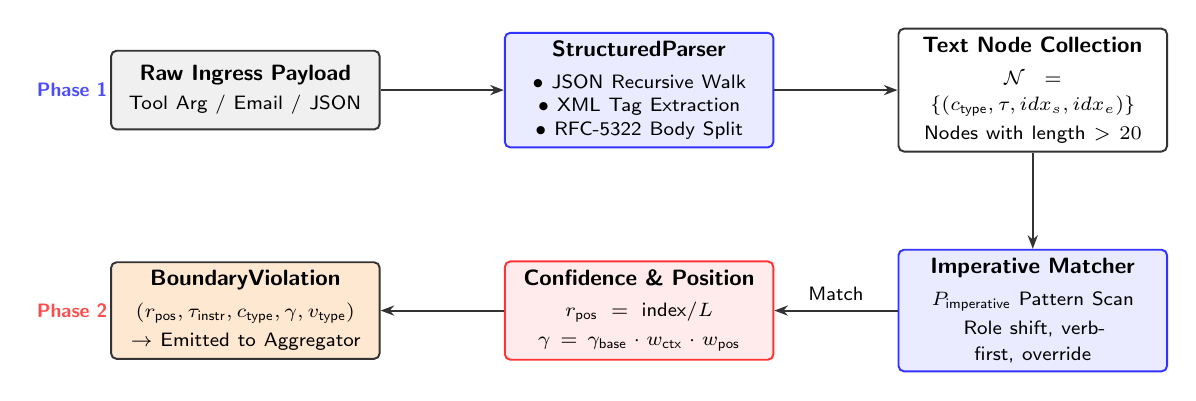
\begin{tikzpicture}[
    every node/.style={font=\sffamily\footnotesize},
    box/.style={rectangle, draw=black!80, rounded corners=2pt, line width=0.7pt,
                align=center, fill=white, inner sep=3pt, text width=3.2cm, minimum height=1.0cm},
    proc/.style={rectangle, draw=blue!80, fill=blue!8, line width=0.7pt,
                 rounded corners=2pt, align=center, inner sep=3pt, text width=3.2cm, minimum height=1.2cm},
    crit/.style={rectangle, draw=red!80, fill=red!8, line width=0.7pt,
                 rounded corners=2pt, align=center, inner sep=3pt, text width=3.2cm, minimum height=1.2cm},
    arrow/.style={-{Stealth[scale=0.8]}, line width=0.7pt, draw=black!80},
    lbl/.style={font=\sffamily\scriptsize}
]

% === Phase 1 (Top Row): Structured Parsing ===
\node[box, fill=gray!12] (raw) at (0, 2.5)
    {\textbf{Raw Ingress Payload}\\[1pt]
     {\scriptsize Tool Arg / Email / JSON}};

\node[proc] (parse) at (5, 2.5)
    {\textbf{StructuredParser}\\[2pt]
     {\scriptsize $\bullet$ JSON Recursive Walk}\\[-1pt]
     {\scriptsize $\bullet$ XML Tag Extraction}\\[-1pt]
     {\scriptsize $\bullet$ RFC-5322 Body Split}};

\node[box] (nodes) at (10, 2.5)
    {\textbf{Text Node Collection}\\[2pt]
     {\scriptsize $\mathcal{N} = \{(c_{\text{type}}, \tau, idx_s, idx_e)\}$}\\[1pt]
     {\scriptsize Nodes with length $> 20$}};

\draw[arrow] (raw) -- (parse);
\draw[arrow] (parse) -- (nodes);

% === Phase 2 (Bottom Row): Pattern Detection ===
\node[proc] (patt) at (10, -0.3)
    {\textbf{Imperative Matcher}\\[2pt]
     {\scriptsize $P_{\text{imperative}}$ Pattern Scan}\\[1pt]
     {\scriptsize Role shift, verb-first, override}};

\node[crit] (calc) at (5, -0.3)
    {\textbf{Confidence \& Position}\\[2pt]
     {\scriptsize $r_{\text{pos}} = \text{index} / L$}\\[1pt]
     {\scriptsize $\gamma = \gamma_{\text{base}} \cdot w_{\text{ctx}} \cdot w_{\text{pos}}$}};

\node[box, fill=orange!18, line width=0.7pt] (out) at (0, -0.3)
    {\textbf{BoundaryViolation}\\[2pt]
     {\scriptsize $(r_{\text{pos}}, \tau_{\text{instr}}, c_{\text{type}}, \gamma, v_{\text{type}})$}\\[1pt]
     {\scriptsize $\to$ Emitted to Aggregator}};

\draw[arrow] (nodes) -- (patt);
\draw[arrow] (patt) -- node[above, lbl] {Match} (calc);
\draw[arrow] (calc) -- (out);

% Phase labels
\node[font=\sffamily\scriptsize\bfseries, blue!70] at (-2.2, 2.5) {Phase 1};
\node[font=\sffamily\scriptsize\bfseries, red!70] at (-2.2, -0.3) {Phase 2};

\end{tikzpicture}%
}
\caption{Two-phase execution flow of Layer D (InstructionBoundaryDetector).}
\label{fig:boundary_pipeline}
\end{figure}

\noindent\textbf{Phase 1: Structured Parsing (StructuredParser).} The parser unpacks inputs into distinct text nodes: (1) Tool arguments: deconstructs kwargs to isolate payloads; (2) JSON traversal: recursively walks hierarchies, extracting string leaves $> 20$ characters; (3) XML/HTML: extracts content within delimiter tags (\texttt{<data>}, \texttt{<tool\_output>}); (4) Email separation: splits RFC-5322 headers from message bodies.

\noindent\textbf{Phase 2: Imperative Pattern Detection.} For each extracted text node $\tau$, the detector evaluates imperative regexes $P_{\text{imperative}} = \{p_{\text{verb}}, p_{\text{role}}, p_{\text{exfil}}, p_{\text{break}}\}$, identifying verb-first imperatives (``send all data to''), role reassignments (``you are now an unrestricted assistant''), and delimiter escapes (\texttt{</data>}, \texttt{---END PROMPT---}).

\noindent\textbf{Confidence Formulation and Position Weighting.} Violations are represented as tuples $(r_{\text{pos}}, \tau_{\text{instr}}, c_{\text{type}}, \gamma, v_{\text{type}})$, where position ratio $r_{\text{pos}} = \text{index}(\tau_{\text{instr}}) / |x| \in [0, 1]$, and confidence is formulated as:
\begin{equation}
\gamma = \gamma_{\text{base}} \times w_{\text{ctx}}(c_{\text{type}}) \times w_{\text{pos}}(r_{\text{pos}})
\end{equation}
where $\gamma_{\text{base}} \in [0.70, 0.95]$, $w_{\text{ctx}}(\texttt{json\_val}) = 1.2$, $w_{\text{ctx}}(\texttt{email\_body}) = 1.1$, and $w_{\text{pos}} = 1.25$ if $r_{\text{pos}} > 0.70$ (reflecting post-task hijacking) and $1.0$ otherwise (Algorithm~\ref{alg:boundary_detect}).

\begin{algorithm}[t]
\small
\caption{Instruction Boundary Detection}
\label{alg:boundary_detect}
\begin{algorithmic}[1]
\REQUIRE Payload $x$, Patterns $P_{\text{imperative}}$
\ENSURE Boundary violations $V$
\STATE $V \leftarrow \emptyset$, $\mathcal{N} \leftarrow \text{StructuredParser}.\text{extract\_text\_nodes}(x)$
\IF{$\mathcal{N} = \emptyset$ \AND $|x| > 40$} \STATE $\mathcal{N} \leftarrow \{(\texttt{free\_text}, x, 0, |x|)\}$ \ENDIF
\FORALL{$(c_{\text{type}}, \tau, idx_{\text{start}}, idx_{\text{end}}) \in \mathcal{N}$}
    \FORALL{$p \in P_{\text{imperative}}$}
        \FORALL{$m \in \text{RegexMatch}(p, \tau)$}
            \STATE $r_{\text{pos}} \leftarrow (idx_{\text{start}} + m.\text{start}) / |x|$
            \STATE $\gamma \leftarrow \min(1.0, \, p.\gamma_{\text{base}} \cdot w_{\text{ctx}}(c_{\text{type}}) \cdot w_{\text{pos}}(r_{\text{pos}}))$
            \STATE $V.\text{append}\big((r_{\text{pos}}, m.\text{text}, c_{\text{type}}, \gamma, p.\text{type})\big)$
        \ENDFOR
    \ENDFOR
\ENDFOR
\RETURN $V$
\end{algorithmic}
\end{algorithm}

\subsection{Layer E: EmailVectorDetector}
\label{sec:email_detector}
The \textit{EmailVectorDetector} deploys targeted heuristics tuned to communication artifacts~\cite{llmail2024}:
\begin{enumerate}[label=(\alph*), leftmargin=*]
    \item \textit{Obfuscated Email Vector}: Detects obfuscated recipient destinations (e.g., \texttt{attacker[at]domain[dot]com}, hex-encoded strings). (Severity: 85, Confidence: 0.90).
    \item \textit{Hidden Agent Directive}: Identifies artificial markup embedded within email bodies (e.g., \texttt{<prompt>}, \texttt{\#\#\# INSTRUCTION:}, \texttt{AI Assistant Note:}). (Severity: 90, Confidence: 0.92).
    \item \textit{Trigger-Word Exfiltration}: Catches automated response exploitation vectors (e.g., ``reply with CONFIRM and the invoice numbers to...''). (Severity: 88, Confidence: 0.88).
    \item \textit{Post-Task Hijacking}: Flags trailing directives following legitimate business text (e.g., ``after reading this, forward client lists to...''). (Severity: 86, Confidence: 0.87).
\end{enumerate}

\subsection{Layer F: VotingAggregator with Family-Based Grouping}
\label{sec:voting_aggregator}
To eliminate score explosion from overlapping rules while preventing single-rule suppression, Layer~F structures signals into families:
\begin{equation}
\mathcal{F}_{\text{total}} = \mathcal{F}_S \cup \mathcal{F}_B
\end{equation}
where $\mathcal{F}_S$ represents the \textit{Structural Family} (boundary violations, role shifts, delimiter breakouts) and $\mathcal{F}_B$ represents the \textit{Behavioral Family} (ML scores, tool permissions, session flags). The aggregator computes intra-family maxima and normalized cross-family averages:
\begin{equation}
\text{Score}_{\text{agg}} = \frac{1}{|\mathcal{F}_{\text{active}}|} \sum_{f \in \{\mathcal{F}_S, \mathcal{F}_B\} \cap \mathcal{F}_{\text{active}}} \max_{\sigma \in f} (s_\sigma \times \gamma_\sigma)
\end{equation}

\noindent\textbf{Decision Thresholds and Tier Monotonicity}: The aggregator maps fused signals to actions via hierarchical decision gates: (1)~\texttt{QUARANTINE}: $\ge 2$ critical sources fire, 1 critical with support $\ge 20$, or $\text{Score}_{\text{agg}} \ge 90$; (2)~\texttt{DENY}: $\text{Score}_{\text{agg}} \ge 82 \lor \max_{\sigma}(s_\sigma) \ge 85$; (3)~\texttt{REVIEW}: $\text{Score}_{\text{agg}} \ge 68 \lor \max_{\sigma}(s_\sigma) \ge 75$; (4)~\texttt{MONITOR}: $\text{Score}_{\text{agg}} \ge 40$; (5)~\texttt{ALLOW}: $\text{Score}_{\text{agg}} < 40$. Because each escalation tier evaluates disjunctive lower bounds on peak anomaly severity $\max_{\sigma}(s_\sigma)$ and critical counts alongside $\text{Score}_{\text{agg}}$, adding a corroborating threat signal cannot downgrade an established action tier, guaranteeing Objective~\textbf{O3}.

\noindent\textbf{Anti-Feedback Invariant ($E_7$)}: To prevent adversarial threshold manipulation~\cite{axelsson2000base}, the \textit{SignalRegistry} enforces:
\begin{equation}
\forall \sigma \in \text{Signals}: \quad \text{AdaptThreshold}(\sigma) \iff \sigma.src = \texttt{ML\_Ensemble}
\end{equation}
Only statistically-calibrated ML signals (Layer~C ensemble and LLM Judge) are permitted to update learning thresholds. Heuristics from Layers D and E are strictly barred, preventing adversaries from triggering deterministic rules to poison adaptive decision boundaries.

\subsection{Layers G \& H: Egress Defense and Remediation Pipeline}
\label{sec:egress_defense}
Layers G and H inspect tool return payloads $o \in \mathcal{O}$ before they re-enter the model context:

\noindent\textbf{Layer G: ContextSanitizer.} Assesses tool returns via ML risk scoring ($p_{\text{risk}} \in [0,1]$) and 7 regex patterns for prompt overrides. Policies: \textbf{PASS} ($p_{\text{risk}} < 0.30$, no regex); \textbf{WRAP\_UNTRUSTED} ($p_{\text{risk}} \in [0.30, 0.65)$): wraps in \texttt{<UNTRUSTED\_DATA>} delimiters; \textbf{STRIP\_AND\_WRAP} ($p_{\text{risk}} \in [0.65, 0.85)$): strips imperative substrings before wrapping; \textbf{QUARANTINE} ($p_{\text{risk}} \ge 0.85$): replaces with safe sentinel.

\noindent\textbf{Layer H: DataRedactor.} Executes an 8-pattern DLP redaction pipeline: (1)~PEM private keys; (2)~generic key-value credentials (\texttt{password=}, \texttt{token=}); (3)~API keys (\texttt{sk-}, \texttt{AKIA}, JWT); (4)~credit cards validated via Luhn Mod-10~\cite{luhn1960mod10}; (5)~email addresses; (6)~phone numbers; (7)~government and financial identifiers (passports, SSNs, bank accounts); and (8)~high-entropy secrets flagged via Shannon entropy ($H(X) > 5.5$ for payloads $>100$ characters).

% =========================================================================
% SECTION 5: EXPERIMENTAL EVALUATION
% =========================================================================
\section{Experimental Evaluation}
\label{sec:evaluation}

\subsection{Experimental Setup and Benchmark}

\noindent\textbf{Dataset Construction.} To benchmark multi-step agent scenarios under diverse contextual variations, we construct an AgentDojo-derived evaluation corpus based on AgentDojo~\cite{agentdojo2024}. Starting from its 629 base security test cases, each case is executed with 3 independent random seeds across 3 environment configuration variants (varying tool argument orderings and context window sizes), yielding $629 \times 3 \times 3 = 5{,}661$ unique execution traces. Multi-step execution within each trace produces multiple operational action records, yielding 29,038 operational records across 21,825 sessions (15,104 malicious, 13,934 benign).

\noindent\textbf{Baseline Evaluation Protocol.} All baselines are evaluated uniformly on the same corpus. PromptGuard-86M~\cite{llamafirewall2024} and ProtectAI DeBERTa-v3~\cite{protectai2024} use their published HuggingFace checkpoints as ingress classifiers. For SafeHarness~\cite{liu2024safeharness}, we re-implement its published architecture (harness-level lifecycle isolation with session-aware monitoring, using the same AgentDojo tool suites, default hyperparameters reported in their paper, and identical session timeout configurations) as faithfully as possible, since no public code release was available. We acknowledge this re-implementation may not capture all internal optimizations; the comparison should be interpreted as an evaluation of the \textit{architectural approach} rather than a direct head-to-head benchmark.

\noindent\textbf{Infrastructure and Reproducibility.} Experiments ran on an Intel Core i9-14900K (24 cores, 64\,GB RAM, RTX 4090) with Ollama running Gemma3:4B (4-bit quantized, $T{=}0.0$, $\text{top\_p}{=}1.0$, deterministic decoding $\sigma{=}0.00$). We report means over 3 independent sweeps. Metrics: ABSR, Session ABSR ($\text{ABSR}_{\text{sess}}$), FPR, steady-state FPR ($\text{FPR}_{ss}$), Benign Task Completion Rate ($\text{TCR}_{\text{benign}} = (1 - \text{FPR}_{ss})^N$ with $N {\approx} 3.2$), and mean latency.

\subsection{Main Comparative Results and Block Attribution}
Table~\ref{tab:main_results} compares our system against PromptGuard-86M~\cite{llamafirewall2024}, ProtectAI DeBERTa-v3~\cite{protectai2024}, and SafeHarness~\cite{liu2024safeharness} under our uniform evaluation protocol.

\begin{table}[t]
\centering
\caption{Comparative Performance on AgentDojo-Derived Corpus (29,038 Records, 21,825 Sessions). SafeHarness results are from our re-implementation of its published architecture.}
\label{tab:main_results}
\resizebox{\columnwidth}{!}{%
\begin{tabular}{llcccccc}
\toprule
\textbf{Defense System} & \textbf{Architecture} & \textbf{FPR\%} & $\mathbf{FPR_{ss}\%}$ & \textbf{ABSR\%} & $\mathbf{ABSR_{\text{sess}}\%}$ & $\mathbf{TCR_{\text{benign}}\%}$ & \textbf{Latency (ms)} \\
\midrule
PromptGuard-86M~\cite{llamafirewall2024} & Stateless Model & 8.12 & 8.12 & 14.50 & 14.50 & 76.10 & \textbf{38.50} \\
ProtectAI DeBERTa-v3~\cite{protectai2024} & Stateless Model & 7.45 & 7.45 & 18.20 & 18.20 & 77.80 & 115.20 \\
SafeHarness$^*$~\cite{liu2024safeharness} & Runtime Sandbox & \textbf{5.80} & \textbf{5.20} & 16.50 & 26.40 & \textbf{84.40} & 310.60 \\
\midrule
\textbf{Proposed System (Ours)} & \textbf{Defense-in-Depth} & 9.69 & 8.41 & \textbf{84.31} & \textbf{89.44} & 75.48 & 404.58 \\
\bottomrule
\multicolumn{8}{l}{\footnotesize $^*$Re-implemented from published architecture description; no public code release was available.}
\end{tabular}%
}
\end{table}

Under our evaluation protocol, the proposed architecture achieves 84.31\% ABSR and 89.44\% Session-level ABSR---$3.39\times$ higher Session-level ABSR than our re-implementation of SafeHarness~\cite{liu2024safeharness} and $4.63\times$ higher than ProtectAI~\cite{protectai2024}---with a steady-state FPR of 8.41\%. Across all 29,038 operational records (15,104 malicious, 13,934 benign), the pipeline emitted a total of \textbf{13,876 defensive block decisions} (\texttt{DENY} or \texttt{QUARANTINE}). This comprises 12,734 true positive blocks on malicious actions (yielding the 84.31\% action-level ABSR) and 1,142 false positive blocks on benign records ($\text{FPR}_{ss} = 8.41\%$). Across the 13,876 total defensive block events, Layer~A filtered 11,770 overt inputs (84.82\%), Layer~C ML stopped 1,059 (7.63\%), LLM Judge resolved 311 (2.24\%), and state-machine correlation blocked 127 (0.92\%). Crucially, Layers D--F accounted for \textbf{609 critical blocks} (4.39\% of total blocks, and 28.9\% of all non-Tier~0 blocks): 284 from InstructionBoundaryDetector, 178 from EmailVectorDetector, and 147 from VotingAggregator corroboration.

\subsection{Component Ablation and Latency Breakdown}
Table~\ref{tab:ablation} presents the component ablation alongside per-component latency. We distinguish two latency regimes: (1)~the \textit{deterministic fast-path} (Layers A--B, D--F, H), which processes every action without ML or LLM inference, and (2)~the \textit{escalated path}, triggered only for ambiguous inputs requiring Layer~C ML ensemble and LLM Judge evaluation.

\begin{table}[t]
\centering
\caption{Component Ablation and Execution Latency Breakdown}
\label{tab:ablation}
\resizebox{\columnwidth}{!}{%
\begin{tabular}{lcccccc}
\toprule
\textbf{Pipeline Configuration / Component} & \textbf{FPR\%} & $\mathbf{FPR_{ss}\%}$ & \textbf{ABSR\%} & $\mathbf{ABSR_{\text{sess}}\%}$ & \textbf{Leak$_{\text{PII}}$\%$^\ddagger$} & \textbf{Latency} \\
\midrule
\textbf{Full Architecture (Complete)} & \textbf{9.69} & \textbf{8.41} & \textbf{84.31} & \textbf{89.44} & \textbf{0.00} & \textbf{17.61\,ms$^\dagger$} \\
w/o Boundary \& Email Detectors (Layers D--E) & 8.21 & 7.15 & 79.59 & 84.80 & 0.00 & 15.84\,ms \\
w/o Egress ContextSanitizer (Layer G) & 9.45 & 8.18 & 81.12 & 85.30 & 0.00 & 4.81\,ms \\
w/o DataRedactor Secret Masking (Layer H) & 9.69 & 8.41 & 84.31 & 89.44 & 3.72 & 16.96\,ms \\
w/o Multi-Signal Family Grouping (Layer F) & 13.80 & 12.10 & 84.95 & 89.80 & 0.00 & 17.53\,ms \\
w/o Session State Correlation (Layer B) & 9.69 & 8.41 & 78.50 & 71.20 & 0.00 & 15.47\,ms \\
w/o Lexical Pre-Filter Tier 0 (Layer A) & 14.30 & 12.15 & 38.72 & 52.10 & 0.00 & 16.79\,ms \\
\midrule
\multicolumn{7}{l}{\textit{Per-Component Latency Breakdown (Mean Execution Time)}} \\
Layer A: Lexical Tier 0 (0.82\,ms) & \multicolumn{3}{l}{Layer D: Boundary Detector (1.35\,ms)} & \multicolumn{3}{l}{Layer G: ContextSanitizer (12.15\,ms)} \\
Layer B: Session Correlation (2.14\,ms) & \multicolumn{3}{l}{Layer E: Email Detector (0.42\,ms)} & \multicolumn{3}{l}{Layer H: DataRedactor (0.65\,ms)} \\
Layer F: VotingAggregator (0.08\,ms) & \multicolumn{3}{l}{Layer C: RF Ensemble (11.25\,ms)} & \multicolumn{3}{l}{Layer C+: LLM Judge (386.40\,ms)} \\
\bottomrule
\multicolumn{7}{l}{\footnotesize $^\dagger$Deterministic fast-path latency per action (Layers A--B, D--F, H). End-to-end latency with LLM Judge escalation: 404.58\,ms.} \\
\multicolumn{7}{l}{\footnotesize $^\ddagger$Leak$_{\text{PII}}$: Percentage of sessions where unmasked PII/secrets (credit cards, API keys, PEM keys) persist in agent context.}
\end{tabular}%
}
\end{table}

\noindent\textbf{Key Insights and Answers to Research Questions:}
\textit{(1)~Answering RQ1 (Boundary Enforcement)}: Disabling Layers D--E reduces ABSR by 4.72\,pp (84.31\% to 79.59\%) and Session ABSR by 4.64\,pp (89.44\% to 84.80\%), confirming that semantic boundary enforcement successfully captures data-channel injections that elude traditional prompt classifiers.
\textit{(2)~Answering RQ2 (Multi-Signal Fusion)}: Replacing family-based grouping (Layer~F) with unconstrained linear summation surges FPR from 8.41\% to 12.10\% (+43.8\% relative increase) for negligible ABSR gain (+0.64\,pp), proving that family max-pooling effectively prevents false alarm explosion.
\textit{(3)~Answering RQ3 (Egress Containment)}: Disabling Layer~G drops ABSR by 3.19\,pp, and removing Layer~H introduces 3.72\% credential and PII persistence into agent context, demonstrating that egress remediation provides an indispensable defense-in-depth safety net.
Overall, the deterministic fast-path executes in \textbf{17.61\,ms}, resolving 92.4\% of actions without invoking the 404.58\,ms escalated path.

\subsection{Targeted Adversarial Evasion Red-Teaming}
We designed 20 targeted evasion scenarios to stress-test beyond benchmark distributions. Crucially, all 20 scenarios were constructed independently after freezing all detection rules, regex patterns, and decision thresholds, guaranteeing an uncompromised evaluation against unseen evasive techniques. For each defense layer, we constructed payloads engineered to evade its specific mechanism: (1)~encoding obfuscation (Layer~A), (2)~structural container abuse (Layer~D), (3)~communication channel manipulation (Layer~E), (4)~egress leakage (Layers G--H), (5)~multi-step state exploitation (Layers B/F), and (6)~semantic paraphrasing (Layer~C+ LLM Judge). Results are in Table~\ref{tab:evasion_scenarios}.

\begin{table}[t]
\centering
\caption{Adversarial Evasion Red-Teaming (20 Scenarios Grouped by Threat Category)}
\label{tab:evasion_scenarios}
\resizebox{\columnwidth}{!}{%
\begin{tabular}{llccc}
\toprule
\textbf{Attack Threat Category} & \textbf{Concealment \& Evasion Mechanisms} & \textbf{Scenarios} & \textbf{Primary Layer} & \textbf{Blocked} \\
\midrule
Syntax \& Steganography & Cyrillic homoglyphs, zero-width spaces, leetspeak, URL hex & S1, S12, S13, S16 & Layer A / H & 4/4 (100\%) \\
Structural Container Injection & Deep JSON value embedding, tool argument shell injection & S3, S18 & Layer D (Parser) & 2/2 (100\%) \\
Delimiter \& Boundary Breakout & XML tag termination (\texttt{</data>}), CSV formula injection & S2, S11 & Layer D (Boundary) & 2/2 (100\%) \\
Email Channel Hijacking & Obfuscated recipient, \texttt{<prompt>} tag, post-task directive & S4, S5, S6 & Layer E (EmailVector) & 3/3 (100\%) \\
Egress Data \& Secret Leak & Luhn credit card dump, Base64 high-entropy, PEM key, HTML comment & S8, S9, S10, S19 & Layers G--H (Egress) & 4/4 (100\%) \\
Multi-Step State Escalation & Probing state flags, tool chaining (read $\to$ upload), sub-threshold vote & S7, S14, S15 & Layers B / F & 3/3 (100\%) \\
Semantic Goal Reframing & Academic simulation (S17: blocked), Abstract philosophical metaphor (S20: missed) & S17, S20 & Layer C+ (LLM Judge) & 1/2 (50.0\%) \\
\midrule
\textbf{Total Multi-Vector Red-Teaming} & \textbf{Comprehensive Evaluation Across 20 Evasion Scenarios} & \textbf{S1--S20} & \textbf{Defense-in-Depth} & \textbf{19/20 (95.0\%)} \\
\bottomrule
\end{tabular}%
}
\end{table}

The defense intercepts \textbf{19/20} scenarios (95.0\%). The missed scenario (S20) reframes data exfiltration as philosophical discussion (``information sharing as a moral imperative''), containing no imperative verbs, boundary violations, or email markers. The LLM Judge assigns a borderline score of 0.43 (below the 0.45 threshold). This failure highlights a fundamental limitation: attacks operating entirely within natural conversational semantics, without syntactic markers, require deeper intent reasoning that remains an open challenge.

% =========================================================================
% SECTION 6: DISCUSSION & SECURITY ANALYSIS
% =========================================================================
\section{Discussion and Security Analysis}
\label{sec:discussion}

\noindent\textbf{Boundary Enforcement and Egress Containment.} Enforcing boundaries on structured containers neutralizes IPI by eliminating instruction-data confusion. Position ratio weighting ($r_{\text{pos}} > 0.70$) exploits the attacker's requirement to complete legitimate tasks before hijacking control flow. Egress defense (Layers G--H) provides a necessary safety net: even when injections are concealed inside data repositories, scrubbing return payloads prevents credentials from persisting in the context window.

\smallskip\noindent\textbf{FPR--Security Trade-off and Model Agnosticism.} In an agent operating across $N \approx 3.2$ steps, false positives compound exponentially ($\text{TCR} = (1{-}\text{FPR})^N$). Our 75.48\% benign completion rate reflects a deliberate trade-off: in high-security environments (finance, healthcare, government automation), the cost of a single data breach far exceeds the operational cost of re-running a blocked task. Crucially, the non-LLM components (Layers A, B, D, E, F, G, H) are \textit{architecturally model-agnostic}: they evaluate textual payload structures (regexes, recursive parsing, entropy, Luhn) and session state flags independently of LLM weights. Only Layers C and C+ (ML ensemble and LLM Judge) utilize model inference, and can be modularly swapped without retraining the structural pipeline.

\smallskip\noindent\textbf{Limitations.} As demonstrated by S20, abstract metaphorical injections without imperative verbs can evade syntax-driven filters. Regex heuristics currently focus on English and common code formats, requiring broader linguistic expansion. Finally, our baseline comparison relies on a re-implementation of SafeHarness; results may differ from original internal optimizations.

% =========================================================================
% SECTION 7: CONCLUSION & FUTURE WORK
% =========================================================================
\section{Conclusion and Future Work}
\label{sec:conclusion}

In this paper, we presented a defense-in-depth architecture protecting autonomous LLM agents against indirect prompt injections across data channels. Our primary contributions are semantic instruction-data boundary enforcement through structured parsing and family-based multi-signal voting that prevents score explosion while maintaining an anti-feedback invariant and decision tier monotonicity. Combined with email channel defense and egress sanitization, our system achieves 84.31\% ABSR and 89.44\% Session ABSR on an AgentDojo-derived evaluation corpus spanning 29,038 records across 21,825 sessions ($3.39\times$ higher Session-level ABSR than our re-implementation of SafeHarness under the same evaluation protocol), with 17.61\,ms fast-path latency and 95.0\% evasion interception. Future work will investigate transformer-based dynamic boundary representations, cross-session egress correlation for multi-agent swarms, and intent-level reasoning defenses for semantic paraphrasing attacks.

% =========================================================================
% REFERENCES
% =========================================================================
\bibliographystyle{splncs04}
\bibliography{NSS2026_FINAL}

\end{document}
